\documentclass[12pt]{article}
\usepackage[utf8]{inputenc}
\usepackage[T1]{fontenc}
\usepackage{amsmath}
\usepackage{amsfonts}
\usepackage{amssymb}
\usepackage{graphicx}
\graphicspath{{image/}}
\usepackage{enumerate}

\title{Data Mining; Assignemt 1}
\author{Name: Jesse Annan \hspace{0.5cm} | \hspace{0.5cm} ID: 002708111}
\date{September 2022}

\begin{document}

\maketitle

\clearpage

\begin{enumerate}[1.]
    \item \begin{enumerate}
        \item[1.1)] \begin{enumerate}[(a)]
            \item Mean = 31.20
            \item Median = 27
            \item Mode = 27
        \end{enumerate} 
    \end{enumerate}

    \item \begin{enumerate}
        \item[2.1)] \begin{enumerate}[(a)]
            \item MIN = 52.30
            \item Q1 = 60.10
            \item Q2 (Median) = 72.60
            \item Q3 = 84.30
            \item MAX = 89.10
        \end{enumerate}

        \item[2.2)] No outliers, this is because per the interquartile range (IQR) rule, no value(s) was 1.5 $\times$ IQR away. The interquartile range is the difference between the Q3 and Q1. \newline \\
        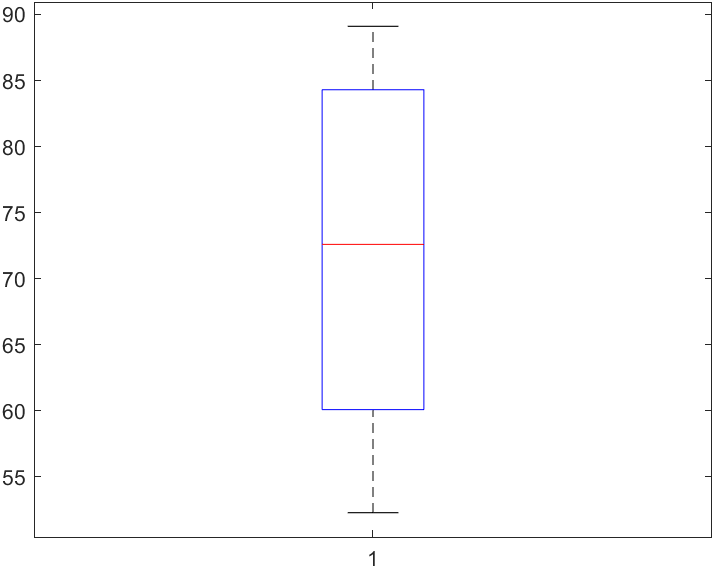
\includegraphics[scale=0.7]{boxplot_q2.png}
        
        \item[2.3)] From the plot we can see that it will be cold during the first and last 3 months of the year, and about room temperature during April and October. The plot also points out that it gets warm from May through September but very warm during July. \newline \\
         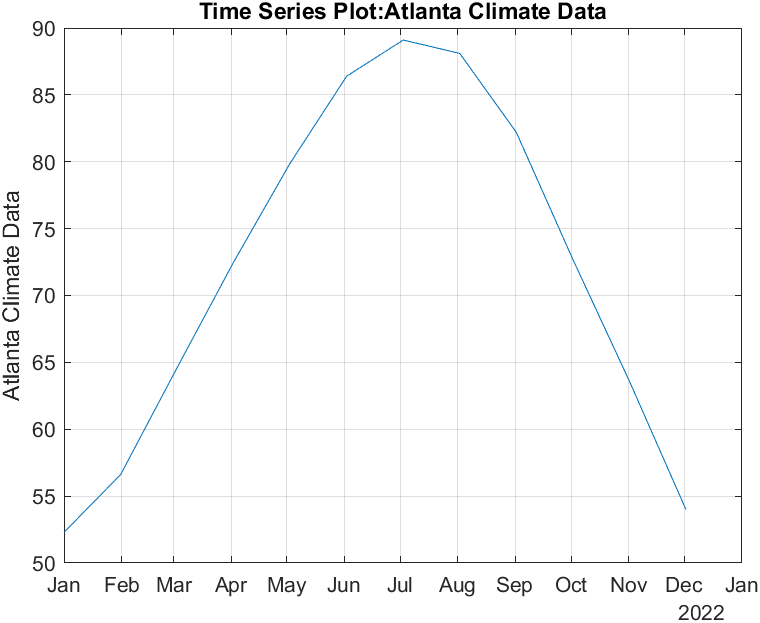
\includegraphics[scale=0.7]{plot_q2.png}
        
    \end{enumerate}

    \item \begin{enumerate}
        \item[3.1)] All are nominal attributes

        \item[3.2)] similarity between "David" and "Susan" \; $S_{David, Susan} = \frac{2}{3} $

        \item[3.3)] similarity between "Susan" and "Lisa" \; $S_{Susan, Lisa} = \frac{1}{3} $
    \end{enumerate}

    \item \begin{enumerate}
        \item[4.1)] All are binary attributes

        \item[4.2)] similarity between "Tom" and "Mat" \; $S_{Tom, Mat} = \frac{4}{4+3+1} = .5 $

        \item[4.3)] similarity between "Mat" and "Lucy" \; $S_{Mat, Lucy} = \frac{3}{3+2+2} = \frac{3}{7} $
    \end{enumerate}

    \item \begin{enumerate}
        \item[5.1)] All are numeric attributes

        \item[5.2)] Pearson's Correlation Coefficient

        \item[5.3)] similarity between "A" and "B" \; $S_{A, B} = 0.7866$

        \item[5.4)] similarity between "B" and "C" \; $S_{B, C} = 0.8331$
    \end{enumerate}
    
\newpage

    \item \begin{enumerate}
        \item[6.1)] All are ordinal attributes

        \item[6.2)] similarity between "Kevin" and "John" \newline \\
        \begin{tabular}{|c|c|} \hline
            \textbf{Kevin} & \textbf{John} \\ \hline
            1 & 0.75 \\
            $\frac{2}{3}$ & 1 \\
            1 & 0.5 \\ \hline
        \end{tabular}

        \item[6.3)] similarity between "John" and "Daniel" \newline \\
        \begin{tabular}{|c|c|} \hline
            \textbf{John} & \textbf{Daniel} \\ \hline
            0.75 & 0.5 \\
            1 & $\frac{1}{3}$ \\
            0.5 & 0 \\ \hline
        \end{tabular}
        
    \end{enumerate}

    \item Normalized Data (min-max normalization) \newline \\
    \begin{tabular}{|c|c|}
        \hline
        \textbf{Patient} & \textbf{Height} \\ \hline
        Tom & 0.4615 \\
        Mat & 0.8462 \\
        Lucy & 0 \\
        Brain & 1 \\ \hline
    \end{tabular}

\end{enumerate}

\end{document}